% Indicate the main file. Must go at the beginning of the file.
% !TEX root = ../main.tex

\chapter{My Awesome Chapter}
\label{chap:4}

\begin{summary}
\colorizee{\lipsum[1]}
\end{summary}

% \localtableofcontents  % Add main table of contents
\clearpage
\markboth{}{}

\section{Introduction}
\label{sec:introduction_acc}

Some text about \gls{qp} optimization in a \gls{mpc} control scheme.  Notice
\gls{mpc} is only shortened the first time. Also, some example
citations~\cite{torresalberto:hal-03621688,torresalberto:hal-04073876,carpentier2019pinocchio}.
Also, check out~\Cref{sec:image1} and later.

\section{Navigation and Notation Aspects in this Manuscript}



On a practical note, a small clarification about navigation is required.


To facilitate navigation throughout this manuscript, every section title
features an arrow on the right that allows quickly going back to the contents
table. This enables going to sections far apart by going through to the table of
contents.


The general outline of the manuscript progressively builds up the methodology
and concepts with each chapter. However, the chapters are intended to be mostly
self-contained. As such, some sections summarize concepts from the previous
ones, to refresh the concepts that are addressed.


On the same note, when definitions are revisited at later stages and it is
deemed relevant to bring it to the reader's attention, it appears on the
manuscript margins like this:
\begin{gather}
  \label{eqn:example1}
  \futurev{eqn:example2}
  \pos \in \coordspace{R}{3}
\end{gather}
where the arrow on the right is a reference to the where it is revisited, right
below:
\begin{gather}
  \label{eqn:example2}
  \prevfuturev{eqn:example1}{eqn:example3}
  \prevrev{eqn:example1}
  \pos = [\poss_x\quad \poss_y \quad \poss_z]
\end{gather}
This allows the reader to quickly go back and forth between both
definitions. This is only used for equations and, less often, for figures.
Sometimes the it indicated that the revisited element (equation or figure) is
exactly the same (for convenience) and sometimes, it indicates that it is
conceptually linked to a previous definition that is extended.

Furthermore, equations are referred with~(equation number) (without explicitely
saying it corresponds to an equation), to facilitate reading. However, when
referring to tables, figures or sections, it is explicitely stated.

Finally, as can be seen in~\labelcref{eqn:example1,eqn:example2}, matrices and
vectors (like~${\pos}$) have a bold font, while scalars use a normal font
(like~${\poss_x,\poss_y,\poss_z}$).

\section{Example Image 1}
\label{sec:image1}
\clearpage
\colorize{some useless text to add space between equations}
\colorize{some useless text to add space between equations}
\colorize{some useless text to add space between equations}
\colorize{some useless text to add space between equations}
\colorize{some useless text to add space between equations}
\colorize{some useless text to add space between equations}

\begin{gather}
  \prevrev{eqn:example2}
  \label{eqn:example3}
  % \tag*{\labelcref{eqn:jacobian} revisited}
  {^W}\twist = {^W}\jac(\q)\qdot \\
  \label{eqn:spatial_acceleration}
  {^W}\twistd = {^W}\jac(\q)\qddot + {^W}\jacdot(\q, \qdot)\qdot
  % \\ \nonumber
  % \text{for}\quad \jac\incoordspace{R}{6\times n}
  % \quad\q,\qdot\incoordspace{R}{n}\quad\twist \in\sethree
\end{gather}




\begin{figure}[tb]
  \centering
  \begin{adjustbox}{width=1\linewidth,center}
  \begin{tikzpicture}[auto, >=latex']
    % We start by placing the blocks
    \node [coordinate, name=input] {};
    \node [block_control, right=1.7cm of input] (planner) {Task-space\\ Dynamic Trajectory\\ Planner};
    \node [block_control, right=2.4cm of planner] (controller) {Dynamic Model\\ Tracking Controller};
    \node [block_model, right=1.5cm of controller,
    node distance=3cm] (robot) {Robot};
    \node [block_model, right=1.5cm of robot,
    node distance=1cm] (human) {Human};
    \node [coordinate, above=.7cm of robot] (dyn_disturb) {};
    \draw [snakearrow] (dyn_disturb) -- (robot) node[pos=0, above] {Unmodeled Dynamics};
    \draw [doublesnakearrow] (robot) -- (human) node[pos=0.5, below=2mm, name=hri] {HRI};

    \node [draw, dashed, align=center, rectangle, above=-7mm of hri, xshift=-4mm,
    minimum height=3.cm,
    minimum width=6.8cm] (dashedd) {};

    % We draw an edge between the controller and system block to
    % calculate the coordinate u. We need it to place the measurement block.
    \draw [->] (controller) -- node[name=u] {} (robot);
    \node [block_env, below=.8cm of controller] (measurements) {Workspace \\ Analysis};

    %%%%% arrows
    \draw [draw,->] (input) -- node[pos=0.5, above, align=center, name=input2] {Target} (planner);
    \draw [->] (planner) -- node[name=des] {Trajectory} (controller);
    \node [below=2cm of input, align=center, xshift=0mm, yshift=0mm] (mpc_freq) {Fast};
    \coordinate[right=0.0cm of mpc_freq] (mpc_arc);
    \draw[->,>=latex'] (mpc_arc) arc[radius=0.5cm,start angle=0,delta angle=-270]; % circle

    % \draw [->] (robot) -- node [name=pose_output] {$\pose$}(output);
    % \draw [-] (robot) |- (measurements);

    \node [coordinate, below left=.4cm of hri] (hri_below) {};
    \draw [->] (hri_below) |- (measurements);
    \node [coordinate, right=1.5cm of hri_below] (hri_rightbelow) {};
    \node [coordinate, below=1cm of hri_rightbelow] (env_disturb) {};
    \draw [snakearrow]
    (env_disturb) -- (hri_rightbelow) node[pos=0, below, align=center] {Environment\\ Dynamics};



    % \draw [->] (measurements) -| node[pos=0.99] {A}
    % node [near end] {$y_m$} (controller);
    \draw [->, dashed] (measurements) -- (controller);
    \draw [->] (measurements) -| node[pos=0.3, below, align=center]
    {Workspace\\ Configuration} node [near end] {} (planner);
    % \draw [->] (measurements) -| node [pos=0.9, align=center, left] {Target} (input2);
    \draw [->] (measurements) -| (input2);
    % \begin{scope}[overlay]
      \node [font = {\normalsize\bfseries}, above of=input, shift={(-.3, .7)},
      anchor=west, align=flush right]
      (title) {Proposed Control Architecture};
    % \end{scope}
  \end{tikzpicture}
  \end{adjustbox}
  \caption{
  \futurev{fig:example2}
    The proposed modular control architecture is based on a cascade loop
    composed of:~1) a task-space Model Predictive Controller (\gls{mpc}) for
    online \mbox{re-planning};~2) a constrained Task Space Inverse Dynamics
    solver to follow the planned trajectory. The whole control loop runs
    synchronously at the control rate.}
  \label{fig:example1}
\end{figure}

\colorizee{\lipsum[2]}

\section{Example Image 2}
\clearpage

\begin{figure}[thpb]
  \centering
  \begin{tikzpicture}
    \begin{axis}[
        % width=12cm,
        height=5cm,
        % axis lines=center,
        axis lines=left,
        no marks,
        scale only axis=true,
        grid=both,
        ylabel style={align=center},
        ylabel style={yshift=0cm,rotate=-90},
        ymax=1.03,
        ymin=-1.03,
        % xmin = 0,
        % xmax= 0.52,
        xlabel=\empty,
        xtick distance={0.1},
        xticklabels={,,},
        scaled y ticks=false,
        scaled x ticks=false,
        ytick pos=left,
        legend pos= outer north east,
        ytick distance={0.2},
        legend cell align={left},
        legend style={at={(1.0,.01)}, anchor=south east, draw=none, fill=none},
        % ylabel=$\twist$ \\ $(\text{m/s})$
        ]
        \addplot[color=forestgreen,ultra thick] table [x=t,y=p,col sep=comma] {data/example_ruckig1.csv};
        \addplot[color=steelblue, ultra thick] table [x=t,y=v,col sep=comma]  {data/example_ruckig1.csv};
        \addplot[color=maroon, ultra thick] table [x=t,y=a,col sep=comma]     {data/example_ruckig1.csv};
        % \addplot[color=forestgreen,line width=2pt] table [x=t,y=p,col sep=comma] {data/example_ruckig1.csv};
        % \addplot[color=steelblue, line width=2pt] table [x=t,y=v,col sep=comma] {data/example_ruckig1.csv};
        % \addplot[color=maroon, line width=2pt] table [x=t,y=a,col sep=comma] {data/example_ruckig1.csv};
        \addlegendentry{$s$}
        \addlegendentry{$\dot{s}$}
        \addlegendentry{$\ddot{s}$}
    \end{axis}
\end{tikzpicture}

  \caption{
  \prevfuturev{fig:example1}{eqn:example3}
  Normalized reference TAP trajectory generated with~\cite{berscheid2021jerk}.
}
  \label{fig:example2}
\end{figure}

\colorizee{\lipsum[3]}

\section{Example Image 3}
\clearpage
\colorizee{\lipsum[4]}

\begin{figure}[thpb]
  \centering
  \begin{tikzpicture}

\draw [-latex] (-2.5,.5) -- (-2.5,6.) ; %y axis
\node at (-2.7,3.) {0};
\draw [-latex](-2.5,3) -- (5.,3) node [anchor = north]{t}; %x axis

\draw (-1.,3) -- (1.,5)  ; %ramp up 2 (deceleration)
\draw (1.,5) -- (2.5,5)  ; % steady
\draw (2.5,5) -- (4.5,3); % ramp down

\draw[pattern=north east lines, pattern color = gray!20]
(-1,3) -- (1.,5) -- (2.5,5) -- (4.5,3) -- (-1,3);
\node at (1.8,3.8) {$ v(t_R) $};


\draw (-2.5,1.5) -- (-1.,3)  ; %ramp up 1 (reversing)
\draw[pattern=north west lines, pattern color = gray!25]
(-2.5,1.5) -- (-1.,3) -- (-2.5,3) -- (-2.5,1.5);
\draw [-stealth](-1.8,1.7) -- (-2.3,2.15);
\node at (-.8,1.7) [anchor = north] {\smaller Acceleration Reversing};



\node at (-2.5,1.5) [anchor = east]{ $ -a_k $ };
\draw (-2.6,1.5) -- (-2.4,1.5);

\node at (-2.5,1) [anchor = east]{ $ -a_M $ };
\draw (-2.6,1) -- (-2.4,1);

\node at (-2.5,5) [anchor = east]{ $ a_M $ };
\draw (-2.6,5) -- (-2.4,5);


\draw [latex -latex] (-2.5,2.9) -- node[anchor = north]{$t_R$} (-1.,2.9);
\draw [latex -latex] (-1.,2.9) -- node[anchor = north]{$t_1$} (1.,2.9) ;
\draw [latex -latex] (1,2.9) -- node[anchor = north]{$t_2$} (2.5,2.9) ;
\draw [latex -latex] (2.5,2.9) -- node[anchor = north]{$t_3$} (4.5,2.9) ;
\draw [latex -latex]  (-2.5,2.45) -- node[anchor = north]{$t_{\text{stop}}$}  (4.5,2.45);

\node [rotate=45] at (-.4,4) {$j_{M}$};
\node [rotate=-45] at (3.9,4) {$-j_{M}$};

\draw [stealth-](1.8,4.6) -- (2.4,5.3);
\node at (2.7,5.3) [anchor = south] {\smaller Deceleration};



\node at (2,1.6) {$\quad t_R \leq t_s$};
\node at (2,1.2) {$-v_k \leq 0 $};
\node at (2,.8) {$-a_k \leq 0 $};

\end{tikzpicture}
  \caption{
  \prevfuturev{fig:example2}{eqn:example4}
    Smooth stopping trajectory with acceleration reversing, where the
    initial velocity and acceleration have the same direction, requiring a
    max-jerk trajectory to inverse the acceleration.}
  \label{fig:example3}
\end{figure}


\section{Example Image 4}
\clearpage
\colorizee{\lipsum[5]}

\begin{figure}[tb]
  \centering
\begin{tikzpicture}
  \robotArm[config={q1=60,q2=-40,q3=-50},
  draw annotations=false,
  % styles={link 1/.style={draw={annotations=false}}}
  ]{3}

  \def\L{1.7}
  \def\axislength{2}
  \def\axiswidth{2}

  \node[forestgreen, scale=\axislength] (S) at (-2,-1.5) {S};
  \draw[forestgreen, <->,line width=\axiswidth]
  (S)++(0.3,2) node[left,scale=0.7*\axislength] {$y$} |-++
  (\L,-\L) node[below,scale=0.7*\axislength] {$x$};

  \node (EE) at (4.61,1.42) {};

  \node[midnightblue, scale=\axislength] (A) at ([shift={(+0.6,+0.5)}] EE) {A};
  \draw[midnightblue,  <->,line width=\axiswidth]
  (EE)++(0,\L) node[left,scale=0.7*\axislength] {$y$} |-++
  (\L,-\L) node[below,scale=0.7*\axislength] {$x$};


  \node[maroon, scale=\axislength] (L) at ([shift={(-0.7,-0.3)}] EE) {L};
  \draw[maroon, rotate around={-120:(EE.north)}, <->,line width=\axiswidth]
  (EE)++(0,\L) node[left,shift={(-0.15, 0)}, rotate=-120,scale=0.7*\axislength] {$y$} |-++
  (\L,-\L) node[below,rotate=-120,scale=0.7*\axislength] {$x$};
\end{tikzpicture}
\caption{
  \prevfuturev{fig:example3}{eqn:example5}
  Depiction of three conventional frames used to describe quantities in
  robotics: S is the world or universal frame; L is a local or body frame; A
  corresponds to a combined frame, placed in the body but aligned with the world
  frame.
}
\label{fig:example4}
\end{figure}

\section{Example Image 5}

\clearpage
\colorizee{\lipsum[6]}


\begin{figure}[tb]
  \centering
  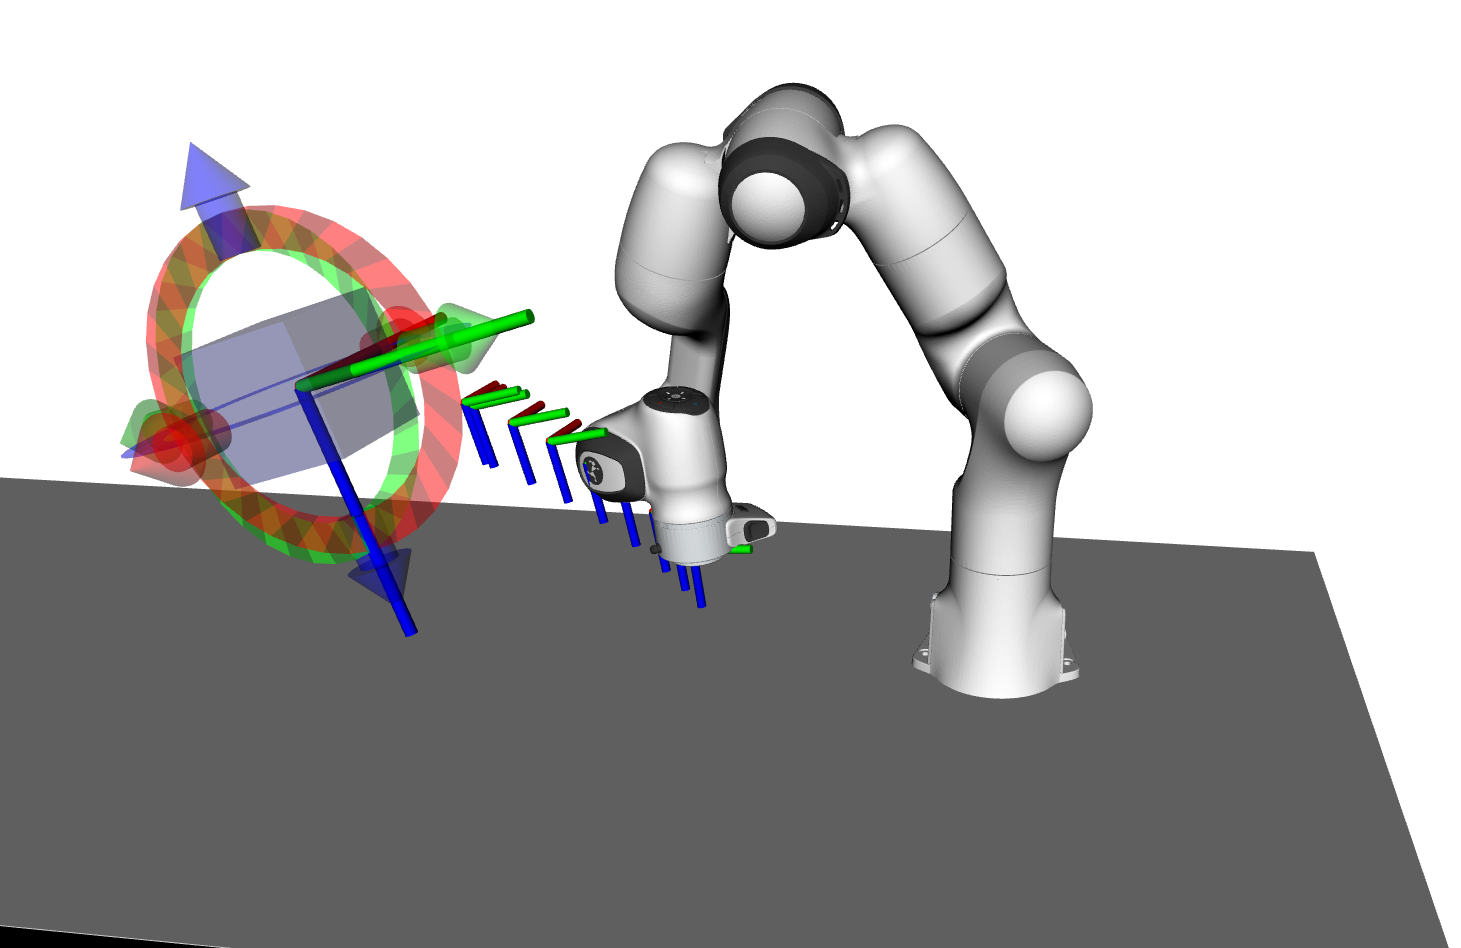
\includegraphics[width=1\linewidth]{Figures/1.png}
\caption{
  \prevrev{fig:example5}
  One final example with a png file.
  }
\label{fig:example5}
\end{figure}
